\section{Winding pressure and essential polygons}
\label{sec:05-pressure}

Throughout the pressure and nesting arguments, except during the explicitly
indicated variation of the loop fugacity, put
\[
 \lambda=\frac{\pi}{8},\qquad \beta=2\lambda=\frac{\pi}{4},
 \qquad \gamma=\frac{\pi}{3\beta}=\frac43,
 \qquad \rho=\frac1{\sqrt{2+\sqrt2}}.
\]
A geometric honeycomb polygon has weight \(\rho^{|P|}\), where
\(|P|\) counts vertices. Polygons are unrooted and unoriented; when
translation classes are used, the translation group will always be specified.

The cylinder exponent concerns polygons separating two marked points.
To obtain a nesting law around one planar point, we must remove two
kinds of polygon with a bounded multiplicative cost: essential polygons
that wind around the cylinder, and contractible polygons too large to fit
near either marker. We treat them separately. The first two derivatives
of an annular pressure control the total essential-polygon weight and
its horizontal-span moment. Section~\ref{sec:05-open-pressure} obtains the planar diameter tail
needed for contractible polygons from a separate open-strip pressure.
Section~\ref{sec:05-nesting} then compares the surviving configurations
with two independent planar nests and derives the strip-length estimates.
The present section supplies the essential-polygon removal bound.

\subsection{The annular transfer and its interpolation data}

Let \(N=2m\), and assign the additive site parameters
\[
 b_1=\cdots=b_m=\lambda/2,
 \qquad b_{m+1}=\cdots=b_{2m}=-\lambda/2.
\]
The auxiliary argument \(z_0=3\lambda/2\) in the column of boxes \(R(z-b_i)\) gives the physical box arguments \(\lambda\) and \(2\lambda\), respectively. In the transfer considered here an essential closed curve receives fugacity \(\chi\), whereas a contractible closed curve receives zero. This convention is specific to the winding pressure.

A state records a cyclic noncrossing partial matching together with a marked complementary region, namely the region containing the past end of the cylinder. Equivalently, draw the matching in a disk with a marked puncture and no strand ending at the puncture. There are finitely many states: an ordinary cyclic noncrossing matching has finitely many regions in which to place the puncture. This information determines composition. Indeed two realizations of the same state decompose the disk into disks and one punctured disk; homeomorphisms of these pieces fixing their boundary arcs identify their sewing rules and distinguish essential from contractible cycles.

Let \(T_\chi(z)\) carry the auxiliary slot around all sites, joining its final output to its initial input. The local identities of the strip calculation apply, since every cycle internal to one of those identities is contractible. At \((\chi,z)=(0,z_0)\), the empty-coordinate functional is invariant and the restriction to vectors with zero empty coordinate has spectral radius less than one. To see the latter assertion in the refined state space, a nonzero diagram with nonempty initial connectivity either closes a killed loop or contains a path joining its two longitudinal cuts. The periodic-slab spanning estimate in Lemma~\ref{lem:02-periodic-slab} therefore gives decay of its powers, exactly as for the unmarked connectivity space. Consequently the eigenvalue \(1\) is simple and strictly dominant, with analytic continuation under small changes of \(\chi\) and of the site parameters.

The matrices \(T_\chi(z)\) commute as \(z\) varies. Insert an invertible crossing between two auxiliary lines, move it through the sites by the three-box identity, and cancel it at the other end; the resulting diagram reverses the two columns. This proves commutation at generic parameters and hence as a rational identity. The simple eigenspace at \(z_0\) is therefore invariant under every \(T_\chi(z)\). Denote its eigenvalue by \(\Lambda(\chi;z)\), normalizing an eigenvector to have empty coordinate one. At \(\chi=0\), the empty-coordinate rule gives \(\Lambda(0;z)=1\).

\begin{lemma}[Annular pinch and analytic data]
\label{lem:05-winding-data}
The function \(\Lambda(\chi;z)\) is rational in \(e^{2iz}\), with denominator dividing \(\prod_i\mathscr D(z-b_i)\), where \(\mathscr D\) is the local denominator in \eqref{eq:E-local-weights}, and tends to \(1+\chi\) at both ends of this multiplicative coordinate. At the balanced specialization it is invariant under \(z\mapsto3\lambda-z\). For \(u=b_i\) and generic remaining sites,
\begin{equation}
 \Lambda(\chi;u+j\lambda)\Lambda(\chi;u)
 =\begin{cases}
   \Lambda(\chi;u+\lambda),&j=2,\\
   1,&j=3.
  \end{cases}
 \label{eq:05-annular-pinch}
\end{equation}
Set \(w=2i(z-z_0)\) and, with derivatives evaluated at \(\chi=0\), define
\begin{equation}
 \begin{gathered}
 f(w)=\partial_\chi\Lambda(\chi;z),\qquad
 h_2(w)=\partial_\chi^2\Lambda(\chi;z),\qquad
 g(w)=h_2(w)-f(w)^2,\\
 (\mathscr L v)(w)=v(w+i\beta)+v(w-i\beta)-v(w).
 \end{gathered}
 \label{eq:05-pressure-derivatives}
\end{equation}
Then \(\mathscr L f\) and \(\mathscr L g\) vanish to orders \(2m,m,m\) at \(0,i\beta,-i\beta\), respectively. The functions \(f-1\) and \(h_2\) are even rational functions of \(e^w\), vanish at both real infinities, and have poles only at the translates of these three knots by \(i\pi\), modulo \(2\pi i\), with the same respective order bounds.
\end{lemma}

\begin{proof}
The common eigenvector is independent of \(z\). Computing the empty output of the transfer on that vector proves the rationality and denominator bound. A shift \(z\mapsto z+\pi\) inserts occupancy signs that cancel around the closed auxiliary. At either imaginary infinity, \(A,U\to0\), \(B\to1\), and all entries remain bounded. Only empty input reaches empty output; it contributes the empty diagram and one essential auxiliary circle, with weights \(1\) and \(\chi\). Reflection reverses the row order and negates all \(b_i\); the balanced list is thereby preserved, and simplicity identifies the reflected eigenline with the original one.

For the pinch, pass the two auxiliaries in order \([u+j\lambda,u]\). At a host with \(x=u-b_k\) their crossing is
\[
 M_x=R_1(x+j\lambda)R_2(x),\qquad
 (I\otimes S_j^{\mathsf t})M_x
   =\widehat R(S_j^{\mathsf t}\otimes I).
\]
At the marked host, \(x=0\) and
\(M_0=(S_j\otimes I)(S_j^{\mathsf t}\otimes I)\).
Close the paired auxiliary trace and move the transpose splitter backwards through all other hosts. At the marked host the remaining contraction is
\[
 (I\otimes S_j^{\mathsf t})(S_j\otimes I)
   =\widehat R\big|_{x=0}.
\]
For completeness, this identity follows by multiplying on the right by \(S_j^{\mathsf t}\otimes I\), using the transposed splitting identity at \(x=0\), and cancelling that factor. Cancellation is valid because \(S_j^{\mathsf t}\) is surjective: insert vacancy, or one through strand into a fixed output and divide by its nonzero coefficient. The fused auxiliary is the one of argument \(u+\lambda\) for \(j=2\), and disappears for \(j=3\). These are identities of annular diagrams, so they prove \eqref{eq:05-annular-pinch} with the essential-loop fugacity retained.

The first two derivatives of \(\log\Lambda\) are \(f\) and \(g\). Taking their derivatives in \eqref{eq:05-annular-pinch} makes \(\mathscr L f\) and \(\mathscr L g\) vanish at the points corresponding to both \(b_i+\lambda\) and \(b_i+2\lambda\). At generic sites the factors giving these zeros are distinct. Analyticity of the normalized eigenvector near the balanced physical sites, and regularity of the boxes at all the evaluation points, permit confluence. The two families give the stated multiplicities. The two sine factors in each \(\mathscr D(z-b_i)\) give the pole list. Since the denominator is independent of \(\chi\), taking two \(\chi\)-derivatives does not increase those orders.
\end{proof}

\subsection{Uniform Hardy-space interpolation}

The interpolation conditions just obtained will estimate the pressure
at the physical point \(w=0\). Their number grows with the cylinder
width, so invertibility alone is insufficient: the inverse must remain
bounded as the knots coalesce and their multiplicities grow. The
following Hardy-space realization separates that issue from the
particular pressure derivatives.

We establish the analytic estimates with constants independent of \(N\). Let \(H\) be the Hardy space on \(|\operatorname{Im}w|<h\), where
\[
 h=\frac{3\beta}{2}=\frac{\pi}{2\gamma}.
\]
Its squared norm is the sum of the squared \(L^2(dx)\) norms on the two boundary lines. With Fourier convention \(\widehat v(k)=\int e^{-ikx}v(x)\,dx\),
\begin{equation}
 \|v\|_H^2=\int_{\mathbb R}2\cosh(3\beta k)
            |\widehat v(k)|^2\,\frac{dk}{2\pi}.
 \label{eq:05-hardy-norm}
\end{equation}
The reproducing kernel is a positive constant times
\(\operatorname{sech}(\gamma(w-\overline v)/2)\).
One way to justify the boundary description is to start with uniformly bounded \(L^2\) norms on interior horizontal lines. The Cauchy--Riemann equation gives their Fourier transforms as \(e^{-ky}\widehat v(k)\) at height \(y\), initially in distributions on compact frequency intervals. Monotone convergence of the resulting weighted integrals gives \eqref{eq:05-hardy-norm} and the two boundary traces.

The prescribed jets determine a finite Hardy model space. We use the
strip form of the standard model-space construction
\cite[Section~1]{Sarason2007}, proving its repeated-zero formulation
directly below. A jet of order \(r\) at a point means the value and the first
\(r-1\) derivatives there. Let \(P_N\) be the orthogonal projection
onto their representing vectors for the three knots in
Lemma~\ref{lem:05-winding-data}, with orders \(2m,m,m\). List their imaginary coordinates, with multiplicities, as \(\theta\), and put
\begin{equation}
 B_N(w)=\prod_\theta
   \frac{e^{\gamma w}-e^{i\gamma\theta}}
        {e^{\gamma w}+e^{-i\gamma\theta}},
 \qquad
 A_N=\gamma^{-1}\log\!\left(\sum_\theta2\cos(\gamma\theta)\right)
     =\gamma^{-1}\log(3N).
 \label{eq:05-blaschke}
\end{equation}
Each factor has modulus one on the boundary and at most one in the strip. Thus multiplication by \(B_N\) is an isometry on \(H\), and
\begin{equation}
 (I-P_N)H=B_NH.
 \label{eq:05-model-space}
\end{equation}
Indeed division by the finite product cancels precisely the specified zeros, preserves boundary norms, and leaves bounded interior \(L^2\) norms. This also proves that the jet space has the asserted dimension.

For \(0<a<1\), define the Fourier multiplier
\begin{equation}
 D_a(k)=
 \frac{\bigl(2\cosh(\beta(k+ia))-1\bigr)\cosh(3\beta k)}
      {\sin(\pi(a-ik))}.
 \label{eq:05-multiplier}
\end{equation}
We use the same symbol for the resulting bounded operator on \(H\).

\begin{lemma}[Coercive jet interpolation]
\label{lem:05-hardy-interpolation}
For every fixed \(0<a<1\), the operators \(D_a\) are bounded and satisfy
\begin{equation}
 \operatorname{Re}D_a(k)\ge c_a>0
 \quad(k\in\mathbb R),\qquad
 \|(P_ND_a|_{P_NH})^{-1}\|\le c_a^{-1}.
 \label{eq:05-coercivity}
\end{equation}
Moreover, writing \(\|\cdot\|_{\partial,p}\) for the sum of the two boundary \(L^p\) norms, one has
\begin{equation}
 \|e^{aw}(1-f)\|_{L^p(\operatorname{Im}w=y)}
       \le C_a e^{aA_N},
 \qquad p=2,4,\quad |y|\le h+\beta.
 \label{eq:05-first-derivative-norms}
\end{equation}
For fixed \(0<a<1/2\),
\begin{equation}
 \bigl|\mathscr Lf(s)\bigr|+
 \bigl|\mathscr Lg(s)\bigr|
 \le C_a|B_N(s)|\bigl(1+e^{2a(A_N-s)}\bigr),
 \qquad s\ge0.
 \label{eq:05-jet-residual}
\end{equation}
For \(\mathscr Lf\) alone, \(2a\) can be replaced by any fixed \(a\in(0,1)\).
\end{lemma}

\begin{proof}
We first solve the jet equation in the Hilbert norm. We then obtain the
fourth-norm estimate needed for the quadratic term \(f^2\), and divide
out the prescribed zeros to estimate the residual.

\paragraph{The jet equation and coercivity.}
Partial fractions for the rational functions in Lemma~\ref{lem:05-winding-data} use derivatives of
\((1+e^{w-i\theta})^{-1}\), up to the specified pole orders, and a constant determined by the limit at positive infinity. That constant vanishes for \(1-f\) and \(h_2\). The beta integral, followed by a pole-free contour shift, gives
\[
 \int_{\mathbb R}\frac{e^{(a-ik)x}}{1+e^{x-i\theta}}\,dx
   =\frac{\pi e^{i\theta(a-ik)}}{\sin\pi(a-ik)}.
\]
Differentiated terms contribute polynomials in \(k\). Weighting by \(e^{aw}\) changes the shift multiplier to \(2\cosh(\beta(k+ia))-1\). Kernel jet vectors have transforms equal to polynomials times \(e^{-k\theta}/\cosh(3\beta k)\). The knot multiset is symmetric, and consequently
\begin{equation}
 e^{aw}\mathscr L(1-f)=D_ax_N,
 \quad x_N\in P_NH,
 \qquad
 e^{aw}\mathscr Lh_2\in D_aP_NH.
 \label{eq:05-partial-fractions}
\end{equation}
All contour shifts used here lie before the first poles of the rational functions.

To check coercivity, symmetry reduces the problem to \(k\ge0\). The real part of \(2\cosh(\beta(k+ia))-1\) is positive. If \(a\ge1/2\), its imaginary part and that of \(\sin\pi(a-ik)\) have the same sign, so the real part of their quotient is positive. If \(a<1/2\), their imaginary parts have opposite signs, but
\[
 \frac{\operatorname{Im}(2\cosh(\beta(k+ia))-1)}
      {\operatorname{Re}(2\cosh(\beta(k+ia))-1)}
 \le\frac{2\sin(\beta a)}{2\cos(\beta a)-1}
 <\tan(\pi a).
\]
The last inequality follows, with \(x=\beta a\in(0,\pi/8)\), by multiplying positive denominators: the difference of the cross-products is \(2\sin(3x)-\sin(4x)>0\). This is sufficient since the absolute ratio of the imaginary and real parts of the denominator is at most \(\cot(\pi a)\). Finally
\[
 D_a(+\infty)=e^{i(\pi/2-3\beta a)},\qquad
 D_a(-\infty)=e^{-i(\pi/2-3\beta a)}.
\]
These limits have positive real part. Continuity proves the uniform lower bound and boundedness. Compressing the real-part inequality to the finite-dimensional jet space proves the inverse bound.

The product defining \(B_N\) gives, throughout the closed strip,
\begin{equation}
 |1-B_N(w)|\le C\min\{1,e^{-\gamma(\operatorname{Re}w-A_N)}\}.
 \label{eq:05-blaschke-tail}
\end{equation}
For large positive real part, sum the deviations of individual factors from one; for the remaining points use \(|B_N|\le1\). It follows by direct integration, for \(p=2,4\), that
\[
 \|e^{aw}(1-B_N)\|_{\partial,p}\le C_a e^{aA_N}.
\]
The jet conditions give the exact interpolation equation
\begin{equation}
 P_ND_ax_N=P_N[e^{aw}(1-B_N)].
 \label{eq:05-first-interpolation}
\end{equation}
Thus \(\|x_N\|_H+\|D_ax_N\|_H\le C_ae^{aA_N}\).

\paragraph{The product estimate.}
The second pressure derivative involves \(f^2\). We therefore need a
fourth-norm estimate in addition to the Hilbert-space bound just proved;
it will control this product without losing a power of \(N\).
Here are the additional bounds needed for products of analytic functions. Embed \(H\) in the two-component boundary space, and let \(\Pi\) be the orthogonal projection onto its traces. In each Fourier fiber it projects onto \((e^{-hk},e^{hk})\). Its diagonal entries differ from the appropriate positive- or negative-frequency projections by bounded square-integrable symbols; its off-diagonal entries decay exponentially. Such remainders map \(L^2\) into \(L^2\cap L^\infty\), hence into \(L^4\). The half-frequency projections are bounded on \(L^4\), the \(p=4\) case of the classical M.~Riesz conjugate-function boundedness theorem; for a real-line reference see~\cite{Grafakos1997,GrafakosSavage2015}. Only boundedness, not a sharp norm, is used here. An elementary proof for real Schwartz data writes its positive-frequency part as \(u+iv\), with \(u\) half the original data. Fourier support gives \(\int(u+iv)^4=0\), whence
\[
 \int v^4\le6\left(\int u^4\int v^4\right)^{1/2}.
\]
The identity is justified first for frequency cutoffs, whose inverse transforms are bounded with \(O(|x|^{-1})\) tails; density and complex linearity then prove the assertion. Therefore \(\Pi\) is bounded from boundary \(L^2\cap L^4\) to itself, with the sum norm.

On the full boundary space,
\[
 P_N=\Pi-B_N\Pi\overline{B_N}.
\]
Boundary multiplication by \(B_N\) preserves every \(L^p\) norm. Hence these projection bounds are uniform in \(N\). Moreover, the commutator of \(P_N\) with any fixed constant diagonal matrix maps \(L^2\) to \(L^4\) uniformly: only the off-diagonal entries of \(\Pi\) occur in its commutator, and multiplication by \(B_N\) commutes with the diagonal matrix.

Let \(D_{\rm edge}\) be the diagonal matrix whose two entries are the limiting values of \(D_a\) in the dominant frequency direction of the corresponding boundary trace. On \(H\), \(D_a-D_{\rm edge}\) maps boundary \(L^2\) to \(L^4\). On each dominant half-axis this follows from exponential convergence of the symbol; on the other half-axis the trace has exponential decay relative to the weighted norm \eqref{eq:05-hardy-norm}. Since \(x_N=P_Nx_N\), the preceding commutator estimate yields
\[
 P_ND_ax_N=D_{\rm edge}x_N+E_N,
 \qquad \|E_N\|_{\partial,4}\le C_a\|x_N\|_H.
\]
The right side of \eqref{eq:05-first-interpolation} has boundary fourth norm at most \(C_ae^{aA_N}\); the diagonal entries of \(D_{\rm edge}\) are nonzero. This proves the same fourth-norm bound on \(x_N\) and on \(D_ax_N\).

Invert the weighted shift multiplier in \eqref{eq:05-partial-fractions}. To move a trace from height \(h\) to height \(h+\beta\), or from \(-h\) to \(-h-\beta\), the multiplier is, up to a constant phase,
\[
 \frac{e^{\pm\beta k}}{2\cosh(\beta(k+ia))-1}.
\]
It has finite constant limits on the two half-axes and exponentially decreasing remainders, so the preceding \(L^2\) and \(L^4\) argument applies. Interior lines follow by the two-boundary Fourier representation. This proves \eqref{eq:05-first-derivative-norms}.

\paragraph{The second derivative and the residual.}
Now fix \(a<1/2\), and write
\(Y_2=e^{2aw}\mathscr Lh_2\in D_{2a}P_NH\).
Since \(\mathscr Lg\) has the prescribed jets,
\begin{equation}
 P_NY_2=P_N[e^{2aw}(\mathscr L(f^2)-B_N)].
 \label{eq:05-second-interpolation}
\end{equation}
If \(v=1-f\), then \(\mathscr L(f^2)=1-2\mathscr Lv+\mathscr L(v^2)\). The second-norm bound at weight \(2a\), the fourth-norm bound at weight \(a\) on the shifted lines, and \eqref{eq:05-blaschke-tail} show that the interpolation input has \(H\)-norm at most \(C_ae^{2aA_N}\). Coercivity gives this bound for \(Y_2\) as well.

Subtract the right interpolation input from each left input in \eqref{eq:05-first-interpolation} and \eqref{eq:05-second-interpolation}. The differences lie in \(B_NH\). Division by \(B_N\) is isometric, and evaluation at a real point has uniformly bounded norm in \(H\). In the first equation the difference is
\(e^{aw}(B_N-\mathscr Lf)\); in the second it is
\(e^{2aw}(\mathscr Lg+B_N)\).
This proves \eqref{eq:05-jet-residual} and its first-derivative variant.
\end{proof}

\subsection{The size and first spatial moment of winding pressure}

We now turn the uniform interpolation estimate into two bounds at the
physical point: the first derivative has order \(N^{-1}\), and the
second logarithmic derivative has absolute value \(O(N^{-1})\).
Their polygon interpretation will then bound the total essential weight
and its first horizontal-span moment.

We will use the inverse of \(\mathscr L\). Its convolution kernel on the real line is
\begin{equation}
 \rho_*(s)=\frac1{\beta\sqrt3}
 \frac{\sinh(2\pi s/(3\beta))}{\sinh(\pi s/\beta)},
 \qquad
 \widehat{\rho_*}(k)=\frac1{2\cosh(\beta k)-1},
 \label{eq:05-resolvent}
\end{equation}
where the quotient at zero is interpreted continuously. This is exactly
the mean density \(\varrho\) from Section~\ref{sec:03-gas-mean}:
it canceled the particle--site sources there, and here it inverts
the shift operator \(\mathscr L\). The Fourier identity follows by a residue computation, or by integrating after the substitution \(u=e^{\beta k}\). In particular
\begin{equation}
 \rho_*(s)>0,\qquad \int\rho_*=1,\qquad
 \rho_*(s)\le Ce^{-\gamma|s|},\qquad
 \lim_{s\to+\infty}e^{\gamma s}\rho_*(s)=\frac1{\beta\sqrt3}.
 \label{eq:05-resolvent-tail}
\end{equation}

\begin{lemma}[Winding pressure bounds]
\label{lem:05-pressure-bounds}
There are constants \(0<c<C<\infty\) such that, for all sufficiently large even \(N\),
\begin{equation}
 \frac cN\le f(0)\le\frac CN,
 \qquad |g(0)|\le\frac CN.
 \label{eq:05-winding-pressure}
\end{equation}
In fact \(e^{\gamma A_N}f(0)\) has a finite strictly positive limit.
\end{lemma}

\begin{proof}
The residual estimate already gives both upper bounds. The lower bound
requires a separate argument: after shifting to the edge
\(A_N=\gamma^{-1}\log(3N)\), we identify a limiting interpolation
problem and show that its contribution at the center is strictly positive.

\paragraph{Upper bounds at the center.}
On the positive real axis the product in \eqref{eq:05-blaschke} satisfies
\begin{equation}
 |B_N(s)|\le\exp\{-c e^{\gamma(A_N-s)}\},\qquad s\ge0.
 \label{eq:05-inner-decay}
\end{equation}
For an individual factor, subtract its squared modulus from one; on \(e^{\gamma s}\ge1\) the result is bounded below by a positive constant times \(e^{-\gamma s}\). Multiplying the factors proves \eqref{eq:05-inner-decay}. The functions \(f,g\) are analytic on a neighborhood of the lines required for \(\mathscr L\) and tend exponentially to constants at both real infinities. Fourier inversion after subtracting those constants therefore gives
\[
 f=\rho_* *\mathscr Lf,
 \qquad g=\rho_* *\mathscr Lg.
\]
By evenness, \eqref{eq:05-jet-residual}, and \eqref{eq:05-resolvent-tail}, their values at zero are bounded by a constant times
\[
 \int_0^\infty e^{-\gamma s}
       e^{-c e^{\gamma(A_N-s)}}
       \bigl(1+e^{2a(A_N-s)}\bigr)\,ds
 \le C e^{-\gamma A_N}=\frac{C}{3N}.
\]
The last inequality follows on substituting \(u=e^{\gamma(A_N-s)}\); the remaining integral is bounded by
\(\gamma^{-1}\int_0^\infty e^{-cu}(1+u^{2a/\gamma})\,du\).

\paragraph{The translated interpolation limit.}
For the lower bound, choose
\(a=\gamma/2\) and \(p=a/\gamma=1/2\).
Translate \(w=A_N+t\) in \eqref{eq:05-first-interpolation} and multiply its unknown and right side by \(e^{-aA_N}\). Expansion of each Blaschke factor, uniformly on compact subsets of the closed strip, gives
\begin{equation}
 B_N(A_N+t)\longrightarrow
 B_\infty(t):=\exp(-e^{-\gamma t}).
 \label{eq:05-inner-limit}
\end{equation}
Indeed the sum of the first-order terms is \(e^{-\gamma t}\), by the definition of \(A_N\), whereas the sum of their squared errors is \(O(N^{-1})\) on compact sets. Both products have boundary modulus one. Their multiplication operators and adjoints converge strongly by dominated convergence, so the boundary projection formula gives strong convergence of the translated projections to
\[
 P_\infty=I-\operatorname{proj}(B_\infty H).
\]
Also \eqref{eq:05-blaschke-tail} supplies an integrable boundary majorant, proving strong convergence in \(H\) of the translated input to \(e^{at}(1-B_\infty(t))\).

For a projection \(P\), extend its compression to
\(P D_aP+(I-P)\) on \(H\). Its real part is bounded below by \(\min(c_a,1)\), as is the real part of its adjoint. It is thus invertible with uniformly bounded inverse, including at \(P=P_\infty\). Write the extended operators as \(\mathcal A_N\) and their strong limit as \(\mathcal A\). The identity
\(\mathcal A_N^{-1}-\mathcal A^{-1}=\mathcal A_N^{-1}(\mathcal A-\mathcal A_N)\mathcal A^{-1}\)
shows strong convergence of their inverses. The normalized unknowns consequently converge to \(x\in P_\infty H\) satisfying
\begin{equation}
 P_\infty D_ax=P_\infty[e^{at}(1-B_\infty(t))].
 \label{eq:05-limit-interpolation}
\end{equation}
Bounded evaluation on the real line implies
\[
 \mathscr Lf(A_N+t)\longrightarrow
 b_\infty(t):=1-e^{-at}(D_ax)(t).
\]
The first-derivative version of \eqref{eq:05-jet-residual} dominates this expression by
\(C e^{-c e^{-\gamma t}}(1+e^{-at})\).
This is integrable after multiplication by \(e^{-\gamma t}\). Hence
\begin{equation}
 \lim_{N\to\infty}e^{\gamma A_N}f(0)
 =\frac{2}{\beta\sqrt3}
     \int_{\mathbb R}e^{-\gamma t}b_\infty(t)\,dt.
 \label{eq:05-pressure-limit}
\end{equation}
Here the original convolution integrates over \(s\ge0\); after translating, its lower endpoint is \(-A_N\), and the same majorant justifies extending by zero and applying dominated convergence.

\paragraph{Strict positivity of the limiting moment.}
The upper estimates have not yet ruled out a zero limit in
\eqref{eq:05-pressure-limit}. To prove strict positivity, we identify the
limiting model space with a half-line space, solve its compressed
multiplier equation by one-sided factorization, and evaluate the
remaining weighted integral. Define
\begin{equation}
 (\mathcal W l)(t)=\int_{\mathbb R}
       \exp\!\left(\frac{v-\gamma t}{2}-e^{v-\gamma t}\right)l(v)\,dv.
 \label{eq:05-laplace-transform}
\end{equation}
It maps \(L^2(dv)\) onto \(H\), with
\[
 \widehat{\mathcal Wl}(\xi)
   =\gamma^{-1}\Gamma(1/2+i\xi/\gamma)
                    \widehat l(\xi/\gamma),
 \qquad
 \|\mathcal Wl\|_H^2=\frac{2\pi}{\gamma}\|l\|_2^2.
\]
These formulas follow by the substitution \(r=e^{v-\gamma t}\) and
\(|\Gamma(1/2+iu)|^2=\pi/\cosh(\pi u)\); alternatively the autocorrelation of the integral kernel is a constant times the reproducing kernel of \(H\). Its nonvanishing Fourier multiplier proves surjectivity.

Writing \(r=e^{-\gamma t}\) and \(y=e^v\) gives
\[
 \mathcal Wl(t)=\sqrt r\int_0^\infty e^{-ry}
                   y^{-1/2}l(\log y)\,dy.
\]
The substitution is an isometry from \(L^2(dv)\) to the data space \(L^2(dy)\). Multiplication by \(B_\infty=e^{-r}\) translates these data to the right by one, with zero extension. Thus \(P_\infty\) corresponds exactly to restriction to \(v<0\). The operator \(D_a\) corresponds to the multiplier \(D_a(\gamma k)\) on the \(v\)-line; denote it by \(\mathcal D\). At \(p=1/2\),
\[
 e^{at}(1-B_\infty)=\mathcal W(e^{pv}\mathbf1_{v<0}),
 \qquad e^{at}=\mathcal W(e^{pv}),
\]
where the second formula is a convergent pointwise integral. Therefore \(l=\mathcal W^{-1}x\) is supported on \(v<0\) and
\begin{equation}
 \mathcal Dl=e^{pv}\quad(v<0),\qquad
 e^{at}b_\infty(t)=\mathcal W(e^{pv}-\mathcal Dl)(t).
 \label{eq:05-half-line-equation}
\end{equation}

We solve this half-line equation by scalar Wiener--Hopf factorization
\cite{WienerHopf1931}. Here the factors can be constructed directly in
the convolution algebra of a delta mass plus an integrable kernel.
At this value of \(a\), the smooth coercive symbol \(D_a(\gamma k)\)
tends to the same positive constant \(1\) at both infinities,
exponentially with all derivatives. The continuous logarithm tending to zero has a Schwartz inverse Fourier transform \(q\). Its conjugation symmetry makes \(q\) real. Split \(q=q_++q_-\) by support on the positive and negative half-lines and exponentiate each piece in the convolution algebra of a delta mass plus \(L^1\). The absolutely convergent series give
\[
 \mathcal D=K_+*K_-,
\]
where \(K_\pm\), and their convolution inverses, are supported on their respective half-lines. For \(s>0\),
\[
 d_+(s):=\int e^{-sv}K_+(dv)
        =\exp\!\left(\int_0^\infty e^{-sv}q(v)\,dv\right)>0.
\]
Since \(K_-*l\) is supported on \(v\le0\), applying the positive-support inverse of \(K_+\) to \eqref{eq:05-half-line-equation} at \(v<0\) gives
\[
 (K_-*l)(v)=d_+(p)^{-1}e^{pv}\mathbf1_{v<0}.
\]
Consequently the residual on the entire line is
\begin{equation}
 e^{pv}-\mathcal Dl
   =d_+(p)^{-1}K_+*(e^{pv}\mathbf1_{v>0}).
 \label{eq:05-positive-residual}
\end{equation}
The half-line identities use ordinary \(L^2\) convolution on the left; on the right they are valid with the displayed exponential weights. Total variation of the \(L^1\) kernels justifies all exchanges below. Integrating \eqref{eq:05-laplace-transform} against \(e^{-(\gamma+a)t}\,dt\), then substituting \(e^{v-\gamma t}\), yields
\begin{align}
 \int_{\mathbb R}e^{-\gamma t}b_\infty(t)\,dt
 &=\frac{\Gamma(3/2+p)}{\gamma}
       \int_{\mathbb R}e^{-(1+p)v}(e^{pv}-\mathcal Dl)(v)\,dv\notag\\
 &=\frac{\Gamma(3/2+p)}{\gamma}
       \frac{d_+(1+p)}{d_+(p)}>0.
 \label{eq:05-positive-moment}
\end{align}
Combining \eqref{eq:05-pressure-limit}, \eqref{eq:05-positive-moment}, and \(e^{\gamma A_N}=3N\) completes the proof.
\end{proof}

\begin{proposition}[Suppression of essential polygons]
\label{prop:05-winding-suppression}
On the balanced cylinder with period \(V=iN\sqrt3/2\), let \([\ell]\) range over simple essential polygons modulo integer horizontal translations, and set \(W(\ell)=\rho^{|\ell|}\). If \(d_x(\ell)\) is their horizontal span, then
\begin{equation}
 \sum_{[\ell]}W(\ell)\asymp N^{-1},\qquad
 \sum_{[\ell]}W(\ell)d_x(\ell)\le C.
 \label{eq:05-winding-moment}
\end{equation}
The total weight of essential polygons separating the two marked points in the balanced two-marker geometry is bounded uniformly in \(N\). At each fixed nonnegative fugacity, deleting all these polygons changes its partition function by at most a bounded multiplicative factor.
\end{proposition}

\begin{proof}
In a slab of \(M\) columns with vacant outer cuts, differentiate the logarithm of the loop partition at \(\chi=0\). Its first derivative counts single essential polygons. Its second derivative is minus the weight of ordered incompatible pairs, including a polygon paired with itself. After division by \(M\), strict spectral dominance gives convergence of the two derivatives to those of \(\log\Lambda(\chi;z_0)\): the spectral projection has nonzero vacuum overlap, equal to one at zero fugacity, and the remaining spectrum decays exponentially, locally uniformly in the analytic parameter. Combinatorially each finite polygon or intersecting pair occupies a finite consecutive interval of columns; its number of placements divided by \(M\) increases to one. Monotone convergence gives
\begin{equation}
 \begin{split}
 f(0)&=\sum_{[\ell]}W(\ell),\\
 -g(0)&=\sum_{[\ell],[\ell']}W(\ell)W(\ell')
        \sum_{j\in\mathbb Z}
          \mathbf1_{\{\ell\cap(\ell'+j)\ne\varnothing\}}.
 \end{split}
 \label{eq:05-cluster-derivatives}
\end{equation}
The physical tiles encode precisely the honeycomb polygons with their vertex weights, and on this embedded trivalent graph intersection is precisely incompatibility.

Let \(\Gamma\) be the triangular translation lattice modulo \(V\). Its integer horizontal subgroup has index \(N\). Fix vertices \(P,Q\) of \(\ell\) of the same bipartite type, with \(\Delta_x=x(Q)-x(P)>0\), and put \(\Delta=Q-P\in\Gamma\). For a translating vector \(a\in\Gamma\), let \(I_P(a)\) indicate that \(P\) lies strictly in the right-hand component of the complement of \(\ell'+a\). Along each horizontal coset it is one on the negative tail and zero on the positive tail. Moreover \(I_Q(a)=I_P(a-\Delta)\). The difference is finitely supported, and
\[
 \sum_{a\in\Gamma}(I_Q(a)-I_P(a))=N\Delta_x.
\]
For an integer horizontal \(\Delta\), this is ordinary telescoping in each of the \(N\) cosets. In general multiply \(\Delta\) by \(N\), which is an integer horizontal translation modulo \(V\), and telescope the sum of the \(N\) translates of the original difference. If the indicators disagree, the path in \(\ell\) from \(P\) to \(Q\) meets \(\ell'+a\); a point on its boundary also gives intersection. Thus at least \(N\Delta_x\) translating vectors give an intersection. Choosing the vertices near the two horizontal extremes, and changing one to a neighbor when necessary to match bipartite types, gives \(\Delta_x\ge d_x(\ell)-C\).

Average the inner intersection count in \eqref{eq:05-cluster-derivatives} over representatives of \(\Gamma/\mathbb Z\). Translation by each representative permutes the horizontal polygon classes and preserves their weights. The resulting inequality is
\[
 f(0)\sum_{[\ell]}W(\ell)(d_x(\ell)-C)\le-g(0).
\]
Now apply Lemma~\ref{lem:05-pressure-bounds}; in particular \(-g(0)\ge0\) by \eqref{eq:05-cluster-derivatives}. This proves \eqref{eq:05-winding-moment}.

Every separating essential polygon meets a fixed arc joining the two markers. That arc has horizontal span \(O(N)\). A polygon class can therefore have at most \(CN+d_x(\ell)+C\) translates meeting it. The two estimates in \eqref{eq:05-winding-moment} bound their total weight. If this bound is \(C\), summing all sets of removed polygons without any compatibility restrictions costs at most \(\sum_{k\ge0}(\chi C)^k/k!=e^{\chi C}\). Positivity provides the opposite inequality by retaining only configurations with no removed polygon.
\end{proof}

\section{Open-strip pressure and the planar polygon tail}
\label{sec:05-open-pressure}

Essential polygons are now controlled. For large contractible polygons
we need a planar estimate, and the next transfer counts all polygons
inside a strip. Let \([P]\) range over unoriented planar polygons modulo all
triangular-lattice translations. Index the triangular bands by integers
and let \(H(P)\) be the difference between the highest and lowest
occupied band indices. Thus \(P\) occupies \(H(P)+1\) bands between
its extremes. The observable to be recovered from the derivative at
zero loop fugacity is
\[
 Q_N=\sum_{[P]}\rho^{|P|}(N-H(P))_+.
\]
The decisive precision is
\(Q_N=c_1N+c_2+O(N^{-1})\): positivity and comparison at two widths
will convert that error into a
\(N^{-2}\) height tail. Here translation classes are taken modulo the
full triangular lattice; this differs from the horizontal classes in
Proposition~\ref{prop:05-winding-suppression}.

\subsection{The variable-fugacity transfer and its boundary terms}

We first derive the transfer identities, including the boundary terms
created by varying the fugacity.

For the transfer construction, vary \(\lambda\) near \(\lambda_0=\pi/8\), and put
\(n=-2\cos(4\lambda)\), \(d=\sin(2\lambda)\).
Thus \(n\) is a local analytic coordinate, since \(dn/d\lambda=8\) at \(\lambda_0\). A closed cycle now receives weight \(n\). Define the raw two-slot box \(r(y)\) by
\begin{equation}
 \begin{aligned}
 e_y&=d\sin(3\lambda)+\sin y\sin(3\lambda-y),
 & A_y&=d\sin(3\lambda-y),\\
 U_y&=d\sin y,
 & B_y&=\sin y\sin(3\lambda-y),\\
 E_y&=\sin(2\lambda-y)\sin(3\lambda-y),
 & F_y&=\sin(y-\lambda)\sin y.
 \end{aligned}
 \label{eq:05-variable-box}
\end{equation}
These are the dilute \(O(n)\) weights listed in
\cite[equation~(1.2)]{ZhouBatchelor1997}, with the common factor
\(\sin(2\lambda)\sin(3\lambda)\) restored.
They are, respectively, the coefficients of vacancy, a single vertical strand, a cup or cap alone, a single diagonal strand, two vertical strands, and a cap together with a cup. Put
\[
 L_y=\sin(2\lambda+y)\sin(3\lambda+y),\qquad
 R_y=r(y)/L_y,\qquad P_y=r(y)/e_y.
\]
At \(\lambda_0\), \(e_y=L_y\), so both normalized boxes coincide with the original box. Use the same splitter diagrams, now with cup coefficients
\(q_2=(2\cos\lambda)^{-1}\), \(q_3=1\), and with occupied-leg coefficient \(q_2\) for \(S_2\).

\begin{lemma}[Local identities away from zero fugacity]
\label{lem:05-variable-algebra}
With \(\widehat P=P_{x+\lambda}\) for \(j=2\), and the identity for \(j=3\),
\begin{equation}
 \begin{gathered}
 R_yR_{-y}=I,\qquad P_{j\lambda}=S_jS_j^{\mathsf t},\\
 (P_x)_2(P_{x+j\lambda})_1(I\otimes S_j)
   =d_j(x)(S_j\otimes I)\widehat P,\qquad
 d_j(x)=1+nq_j\frac{A_{x+j\lambda}U_x}
                          {e_{x+j\lambda}e_x}.
 \end{gathered}
 \label{eq:05-variable-splitting}
\end{equation}
The raw boxes also satisfy the three-box Yang--Baxter identity.
\end{lemma}

\begin{proof}
For unitarity, the one-occupancy sector is the two-by-two matrix with diagonal \(A\) and off-diagonal \(B\). Direct substitution in \eqref{eq:05-variable-box} gives its inverse after normalization by \(L_yL_{-y}\). In the even-occupancy sectors the required identities are
\[
 \begin{gathered}
 e_ye_{-y}+nU_yU_{-y}=E_yE_{-y}=L_yL_{-y},\\
 e_{-y}U_y+(E_y+nF_y)U_{-y}=0,\\
 E_yF_{-y}+F_yE_{-y}+nF_yF_{-y}+U_yU_{-y}=0.
 \end{gathered}
\]
They prove \(R_yR_{-y}=I\). The factorization at \(j\lambda\) follows by substituting \(y=2\lambda,3\lambda\).

We record the coefficient check for splitting to retain the terms arising from the nonzero cycle weight. In the following tables, subscript \(1\) means argument \(x+j\lambda\), subscript \(2\) means argument \(x\), and every letter has been divided by the corresponding \(e\). Unsubscripted letters belong to \(\widehat P\); for deletion take \(B=1\) and the other nonempty two-slot coefficients zero. Write \(q=q_j\) and \(k=q_2\) for \(j=2\), \(k=0\) for \(j=3\). Outputs are numbered \(1,2,3\), with \(1,2\) the split slots; a parenthesized pair denotes an additional cup. In the last block a parenthesized output pairs the two input strands, whereas an unparenthesized pair denotes through strands. The coefficient equalities are
\[
\begin{array}{c|c|c|c}
\text{input}&\text{output}&\text{two boxes}&\text{fused value}\\\hline
00&\varnothing&d_j&d_j\\
&12&U_1A_2+qB_1B_2&d_jq\\
&13&U_1B_2+qB_1A_2&d_jkU\\
&23&U_2+qA_1(E_2+nF_2)&d_jkU\\\hline
10&1&A_1+q(F_1+nE_1)U_2&d_jkA\\
&2&B_1A_2+qU_1B_2&d_jkA\\
&3&B_1B_2+qU_1A_2&d_jB\\
&3,(12)&qF_1E_2&d_jqB\\
&1,(23)&A_1U_2+q(E_1E_2+F_1F_2+nE_1F_2)&0
\end{array}
\]
and, for \(j=2\),
\[
\begin{array}{c|c|c|c}
01&1&k(B_1+U_1U_2)&d_2kB\\
&2&k(A_1A_2+B_2)&d_2kB\\
&3&k(A_1B_2+A_2)&d_2A\\
&1,(23)&k(B_1U_2+U_1F_2)&0\\
&3,(12)&kU_1E_2&d_2qA\\\hline
11&\varnothing&k(U_1+B_1U_2)&d_2U\\
&12&k(E_1A_2+A_1B_2)&0\\
&(12)&kF_1A_2&d_2qU\\
&13&k(E_1B_2+A_1A_2)&d_2kE\\
&(13)&kF_1B_2&d_2kF\\
&23&kB_1E_2&d_2kE\\
&(23)&k(U_1U_2+B_1F_2)&d_2kF
\end{array}
\]
The terms proportional to \(n\) are exactly the closed cups in the contraction. These tables can be verified without diagrammatic simplifications: put \([s]=T^s-T^{-s}\), \(T=e^{i\lambda}\), and \(p=x/\lambda\). At argument \(x+l\lambda\), the normalized tuple \((A,B,U,E,F)\) is
\[
 \frac{([2][3-p-l],\,[p+l][3-p-l],\,[2][p+l],\,
         [3-p-l][2-p-l],\,[p+l-1][p+l])}
      {[2][3]+[p+l][3-p-l]}.
\]
Substitute \(q_2=[1]/[2]\), \(n=-(T^4+T^{-4})\), and clear denominators. Multiplication gives the displayed right columns, proving all occupancy sectors of \eqref{eq:05-variable-splitting}.

For the three-box identity, specialize its second argument to \(y=j\lambda\), \(j=2,3\). Splitting, transposition, and reflection reduce both sides to the same fused diagram with scalar \(d_j(x)\). Unitarity gives the further specializations \(y=j\lambda-x\); \(y=0\) follows from \(R_0=I\). After clearing scalar denominators, each occupancy component has exponents between \(-4\) and \(4\) in \(e^{iy}\), all of fixed parity. The five values modulo \(\pi\) just listed therefore determine the polynomial at generic \(x\), and rational continuation proves the identity everywhere it is defined.
\end{proof}

Let \(x_i\) be host arguments near \(\lambda/2\), and use the notation
\[
 \bar z=3\lambda-z,
 \qquad \mathfrak m(z)=\frac{\sin(3\lambda/2-z)}{\sin(3\lambda/2+z)},
 \qquad K(a)=\text{vacancy}+a\,\text{cup}.
\]
The bar here denotes this affine reflection, not complex conjugation. Define an open transfer \(t(z)\) on ordinary disk states by passing auxiliaries \([\bar z,z]\), the rightmost crossing each host first, with normalized box \(P_{\text{auxiliary}-\text{host}}\). Insert \(K(\mathfrak m(\bar z))\) at the bottom and contract with \(K(\mathfrak m(z))^{\mathsf t}\) at the top.
Figure~\ref{fig:05-open-transfer} records the auxiliary order and the
boundary tensors. The caps are part of the transfer: they contribute
the two scalar factors when auxiliaries are fused.

\begin{figure}[!hbp]
\centering
\begin{tikzpicture}[scale=1,every node/.style={font=\small}]
 \foreach \x/\lab in {-1/{\bar z},1/{z}} {
   \draw[blue!60!black,thick,->] (\x,.15)--(\x,4.3);
   \node[above] at (\x,4.3) {$\lab$};
 }
 \foreach \y/\lab in {1/{x_1},2/{x_k},3/{x_N}} {
   \draw[->] (2.6,\y)--(-2.5,\y);
   \node[right] at (2.6,\y) {$\lab$};
   \foreach \x in {-1,1} {
      \fill[white] (\x-.16,\y-.16) rectangle (\x+.16,\y+.16);
      \draw (\x-.16,\y-.16) rectangle (\x+.16,\y+.16);
   }
 }
 \node at (2.2,2.5) {$\vdots$};
 \node at (2.2,1.5) {$\vdots$};
 \draw[dashed,thick] (-1,.15) to[out=-90,in=-90] (1,.15);
 \draw[dashed,thick] (-1,3.8) to[out=90,in=90] (1,3.8);
 \node[below] at (0,-.4) {$K(\mathfrak m(\bar z))$};
 \node[above] at (0,4.5) {$K(\mathfrak m(z))^{\mathsf t}$};
 \node[left,align=right] at (-2.5,2) {host lines};
\end{tikzpicture}
\caption{The open transfer, drawn as an operator diagram rather than a
physical embedding. The ordered auxiliaries are \([\bar z,z]\), so the
rightmost line crosses each host first; each box has argument auxiliary
minus host. A dashed boundary arc denotes the tensor
\(K(a)=\text{vacancy}+a\,\text{cup}\), not a compulsory occupied arc.
At \(z=\bar z=3\lambda/2\) both cup coefficients vanish, leaving the
two physical columns with vacant auxiliary boundaries.}
\label{fig:05-open-transfer}
\end{figure}


\begin{lemma}[Open transfer and its pinches]
\label{lem:05-open-pinch}
The matrices \(t(z)\) commute and are invariant under \(z\leftrightarrow\bar z\). At \(\lambda=\lambda_0\), \(x_i=\lambda/2\), and \(z=3\lambda/2\), this is the transfer of two physical columns with vacant auxiliary boundaries. Its simple eigenvalue continuing \(1\) will be denoted by \(\Lambda_o(n;z)\). It is rational and \(\pi\)-periodic in \(z\), equals one at \(n=0\), and tends to \(1+n\) at both imaginary infinities. For \(u=x_i\), \(v=u+j\lambda\), its pinch rule is
\begin{equation}
 \Lambda_o(n;v)\Lambda_o(n;u)
 =c_bc_t\prod_kd_j(u-x_k)d_j(\bar v-x_k)
 \begin{cases}
 \Lambda_o(n;u+\lambda),&j=2,\\
 1,&j=3,
 \end{cases}
 \label{eq:05-open-pinch}
\end{equation}
where \(w_0=u+v-3\lambda\) and
\begin{equation}
 c_b=\frac{e_{w_0}+nq_j\mathfrak m(\bar u)A_{w_0}}{L_{w_0}},
 \qquad
 c_t=\frac{e_{-w_0}+nq_j\mathfrak m(v)A_{-w_0}}{L_{-w_0}}.
 \label{eq:05-boundary-scalars}
\end{equation}
\end{lemma}

\begin{proof}
Exchanging adjacent auxiliaries \(v,u\) uses the crossing \(R_{v-u}\) at the bottom, moved to the top by the three-box identity. For exchanging the two lines of one transfer, the boundary identity is
\[
 R_{\bar z-z}K(\mathfrak m(\bar z))
   \ \text{is proportional to}\ K(\mathfrak m(z)).
\]
The proportionality follows from, at \(y=\bar z-z\),
\[
 U_y+\mathfrak m(\bar z)(E_y+nF_y)
 =\mathfrak m(z)(e_y+n\mathfrak m(\bar z)U_y).
\]
The transposed inverse crossing contributes the reciprocal scalar, proving reflection symmetry.

For two pairs, the exchanges taking
\([\bar v,v,\bar u,u]\) to \([\bar u,u,\bar v,v]\) have operator product
\[
 (R_{-w_0})_2(R_h)_3(R_{-h})_1(R_{w_0})_2,
 \qquad h=v-u,\quad w_0=v+u-3\lambda,
\]
with the rightmost factor acting first. They take the product of bottom caps exactly to its reversal. By unitarity, this reduces to left-right symmetry of
\((r(h))_3(r(w_0))_2[K(a)\otimes K(b)]\),
where \(a=\mathfrak m(\bar v)\), \(b=\mathfrak m(\bar u)\). Only the paired output types \(12,34\) and \(13,24\) need comparison; their equalities are
\begin{equation}
 \begin{aligned}
 aA_{w_0}e_h+ab(nE_{w_0}+F_{w_0})U_h
   &=e_{w_0}U_h+bA_{w_0}(E_h+nF_h),\\
 (a-b)B_{w_0}A_h&=(1-ab)U_{w_0}B_h.
 \end{aligned}
 \label{eq:05-cap-exchange}
\end{equation}
Substitution from \eqref{eq:05-variable-box} and the sine formula for \(\mathfrak m\) proves them. Replacing \(v,u\) by \(\bar u,\bar v\) and transposing gives the top exchange, hence commutation.

At the physical center both cap coefficients vanish. Spectral simplicity of the open-strip transfer gives an analytic simple eigenspace nearby, invariant under all \(t(z)\) by commutation. The empty-coordinate rule at \(n=0\) makes its eigenvalue identically one. At imaginary infinity, \(A_y/e_y,U_y/e_y\to0\), \(B_y/e_y\to1\), and \(\mathfrak m(z)\mathfrak m(\bar z)\to1\). Thus the empty-output computation is \(1+n\). Occupancy signs prove periodicity, and computing on the fixed common eigenvector proves rationality.

For the pinch, exchange the middle lines using \(R_{w_0}\) on the bottom caps and \(R_{-w_0}\) on the top, reaching order \([\bar v,\bar u,v,u]\). The descending pair \(v,u\) crosses first. At host \(x_i=u\), the factorization of \(P_{j\lambda}\), together with \(P_0=I\), inserts a transpose splitter at input. Move it backwards through the other hosts by the transposed version of \eqref{eq:05-variable-splitting}. Its contraction against the exchanged bottom caps splits the first pair by \(S_j\), with scalar \(c_b\). In raw coefficients the necessary identities are
\begin{equation}
 \begin{aligned}
 aA_{w_0}+q_jab(nE_{w_0}+F_{w_0})
   &=q_j(e_{w_0}+nq_jbA_{w_0}),\\
 aB_{w_0}+abU_{w_0}
   &=U_{w_0}+bB_{w_0}\\
   &=\mathfrak m(\bar u-\lambda)
                  (e_{w_0}+nq_jbA_{w_0})\quad(j=2).
 \end{aligned}
 \label{eq:05-cap-fusion}
\end{equation}
Here \(a=\sin(v-3\lambda/2)/\sin(9\lambda/2-v)\), and likewise for \(b\); multiplying out proves \eqref{eq:05-cap-fusion}, just as for \eqref{eq:05-cap-exchange}. Move the first pair's splitter through the hosts by the reflected splitting identity. The reflected top calculation, with \(\bar u,\bar v\), gives \(c_t\). The remaining descending pair has both an input and output transpose splitter; transposed intertwining reduces it to the other fused transfer. Cancelling the surjective input splitter is valid as in the annular proof. Every crossed host contributes the two factors displayed in \eqref{eq:05-open-pinch}. This proves that identity for generic other sites, hence by continuation.
\end{proof}

\subsection{The forced interpolation problem}

We have obtained the open transfer and its exact boundary scalars.
We next differentiate its pinches to identify the forced interpolation
problem whose value at the physical center is the planar polygon
pressure. Define \(F_o(z)=\partial_n\Lambda_o(n;z)|_{n=0}\). In all formulas that follow, raw coefficients and auxiliary arguments are evaluated at \(\lambda_0\). Movement of evaluation arguments while differentiating costs nothing, because \(\Lambda_o(0;z)\) is constant. Introduce
\begin{equation}
 \begin{aligned}
 \phi_j(x)&=q_j\frac{U_xA_{x+j\lambda}}{e_xe_{x+j\lambda}},\\
 b_j(u)&=-\frac{U_{w_0}U_{-w_0}}{e_{w_0}e_{-w_0}}
  +q_j\left[
      \mathfrak m(\bar u)\frac{A_{w_0}}{e_{w_0}}
      +\mathfrak m(u+j\lambda)\frac{A_{-w_0}}{e_{-w_0}}
       \right],\qquad w_0=2u+(j-3)\lambda.
 \end{aligned}
 \label{eq:05-open-forcing}
\end{equation}
The first term of \(b_j\) comes from differentiating scalar unitarity on the vacuum sector. Formula~\eqref{eq:05-open-pinch} gives the remaining terms.

There is one additional evaluation. At \(z=0\), the top cap has \(\mathfrak m(0)=1\) and folds the two columns into one another. A quarter-turn of a raw box changes its argument to \(3\lambda-y\), and \(e_y=e_{3\lambda-y}\). Each folded pair therefore cancels by unitarity at \(x_k,-x_k\), contributing
\(1+nU_{x_k}U_{-x_k}/(e_{x_k}e_{-x_k})\); the remaining bottom factor is \(1+n\mathfrak m(3\lambda)\). Hence
\begin{equation}
 F_o(0)=\mathfrak m(3\lambda)
            +\sum_k\frac{U_{x_k}U_{-x_k}}{e_{x_k}e_{-x_k}}.
 \label{eq:05-folded-value}
\end{equation}
At \(8\lambda=\pi\), direct sine identities give
\begin{equation}
 \begin{gathered}
 \phi_3(x)=\phi_2(x)+\phi_2(x+\lambda),\qquad
 b_3(u)=b_2(u)+b_2(u+\lambda),\\
 b_2(\lambda)=\mathfrak m(3\lambda),\qquad
 \phi_2(\lambda-x)+\phi_2(-x)
       =\frac{U_xU_{-x}}{e_xe_{-x}}.
 \end{gathered}
 \label{eq:05-forcing-identities}
\end{equation}
Combining the two differentiated pinches using \eqref{eq:05-forcing-identities} shows that the even residual
\[
 F_o(z+\lambda)+F_o(z-\lambda)-F_o(z)
 -\sum_k[\phi_2(z-\lambda-x_k)+\phi_2(2\lambda-z-x_k)]
 -b_2(z-\lambda)
\]
vanishes at \(z=x_i+\lambda,x_i+2\lambda\) and their reflections about \(3\lambda/2\). Formula~\eqref{eq:05-folded-value} gives zeros at \(z=\lambda,2\lambda\) as well.

Now set every \(x_i=\lambda/2\) and use \(s=2i(z-3\lambda/2)\). To distinguish the physical center from the folded evaluation
\eqref{eq:05-folded-value}, write
\[
 \mathcal F_o(s)=F_o(3\lambda/2+s/(2i)).
\]
Thus \(\mathcal F_o(0)\) is the pressure derivative at the physical
center \(z=3\lambda/2\), while \(F_o(0)\) in
\eqref{eq:05-folded-value} is the folded value at \(z=0\). Set
\begin{equation}
 Y(s)=\mathscr L\mathcal F_o(s)-N\phi(s)-b(s),\qquad
 \phi(s)=\phi_2(y)+\phi_2(-y),\quad
 b(s)=b_2(\lambda/2+y),\quad y=s/(2i).
 \label{eq:05-open-residual}
\end{equation}
Confluence yields zeros of orders \(2N,N,N\) at \(0,i\beta,-i\beta\), and simple zeros at \(\pm i\beta/2\). The function \(\mathcal F_o\) is even, rational in \(e^s\), tends to one at both real infinities, and has poles of orders at most \(N+1\) at \(\pm3i\beta\), and \(2N\) at \(4i\beta\), modulo \(2\pi i\). These bounds count the two box denominators per host and the two boundary denominators. Differentiation does not increase the cleared denominator at zero fugacity: if \(A(n,s)/D(n,s)\) equals one at \(n=0\), its derivative is \((A_n-D_n)/D\) there.

Both forcing terms are rational in \(e^s\) and are \(O(e^{-|\operatorname{Re}s|})\) at real infinity. The function \(\phi\) is analytic in a neighborhood of \(|\operatorname{Im}s|\le h\), and \(b\) has at most simple poles at the two boundary points \(\pm ih\). To check the possibly closer poles of \(b\), use the raw coefficients at \(y=\lambda\):
\[
 \frac{U_{-2\lambda}}{A_{-2\lambda}}
    =\frac{\sin(-2\lambda)}{\sin(5\lambda)}
    =\mathfrak m(7\lambda/2),\qquad
 \frac{U_{2\lambda}}{e_{2\lambda}}=q_2.
\]
The two singular terms at \(y=\lambda\) cancel; reflection gives the cancellation at \(-\lambda\). This cancellation is independent of the hosts. Thus all preceding evaluations and coalescences, including the shifted \(\mathcal F_o\) terms, occur at regular points.

\begin{lemma}[Open-strip interpolation estimate]
\label{lem:05-open-interpolation}
For some fixed \(a\in(\gamma/2,1)\), and uniformly in \(N\),
\begin{equation}
 |Y(s)|\le C e^{-cNe^{-\gamma s}}
               (1+N^{a/\gamma}e^{-as}),\qquad s\ge0.
 \label{eq:05-open-error}
\end{equation}
Consequently
\begin{equation}
 \mathcal F_o(0)=(\rho_* *(N\phi+b))(0)+O(N^{-1}).
 \label{eq:05-open-center}
\end{equation}
\end{lemma}

\begin{proof}
The poles of \(\mathcal F_o-1\) determine the space of unknowns, whereas
zeros of \(Y\) determine the interpolation equations. These spaces have
the same dimension but different two-dimensional additions to their
common base. We first show that the resulting interpolation remains
uniformly invertible. We then remove the bulk forcing \(N\phi\), treat
the two boundary poles of \(b\), and estimate what remains.

\paragraph{The unknown and equation spaces.}
Use the Hardy space \(H\) on \( |\operatorname{Im}s|<3\beta/2\),
with norm \eqref{eq:05-hardy-norm}, and the multiplier \(D_a\) in
\eqref{eq:05-multiplier}. Let \(P\) project
onto the base jets of orders \(2N,N,N\) at \(0,i\beta,-i\beta\).
Let \(P'\) increase the two outer orders by one, and let \(P''\) instead
add the simple knots \(i\beta/2,-i\beta/2\). Their complementary inner
functions are \(B,B',B''\), respectively. The extra orders of \(P'\)
come from the two boundary denominators of the transfer; the extra knots
of \(P''\) come from the folded evaluation \eqref{eq:05-folded-value}.
Partial fractions, as in \eqref{eq:05-partial-fractions}, give
\begin{equation}
 e^{as}\mathscr L(\mathcal F_o-1)=D_ax,\qquad x\in P'H.
 \label{eq:05-open-partial-fractions}
\end{equation}
We first prove that
\begin{equation}
 P''D_a:P'H\longrightarrow P''H
 \quad\text{has inverse norm bounded independently of }N
 \label{eq:05-open-inverse}
\end{equation}
for all sufficiently large \(N\) and all \(a\) in a fixed neighborhood of \(\gamma/2\).

At \(a=\gamma/2\), the compression to \(PH\) is uniformly invertible by \eqref{eq:05-coercivity}, and \(D_a(k)\to d_0=1\) at both frequency infinities. The orthogonal decompositions of the two enlarged spaces are
\[
 P'H=PH\oplus B E',\qquad P''H=PH\oplus B E'',
\]
where \(E'\) and \(E''\) are the fixed two-dimensional jet spaces at \(\pm i\beta\) and \(\pm i\beta/2\), respectively. For each fixed vector \(e\) in either space,
\[
 \|(D_a-d_0I)Be\|_H+
 \|(D_a^*-d_0I)Be\|_H\longrightarrow0.
\]
Indeed \(B(s)\to0\) boundedly at every real point, so \(Be\to0\) in real-line \(L^2\) by domination. Its weighted Fourier mass on a fixed compact interval consequently tends to zero. Outside that interval \(D_a-d_0\) is uniformly small, while \(\|Be\|_H=\|e\|_H\). The same argument applies to the adjoint; finite dimensionality makes convergence uniform on unit balls. The off-diagonal blocks of \(P''D_a|_{P'H}\) therefore tend to zero, and its extra block tends to \(d_0\) times the overlap projection from \(E'\) to \(E''\). The cross-Gram matrix of the kernel-vector bases is, up to the fixed positive kernel constant,
\[
 \begin{pmatrix}
 \sec(\pi/4)&\sec(\pi/12)\\
 \sec(\pi/12)&\sec(\pi/4)
 \end{pmatrix},
 \qquad \det=2-\sec^2(\pi/12)>0.
\]
Thus the limiting extra block is invertible. The block inverse proves \eqref{eq:05-open-inverse} at \(a=\gamma/2\). Operator-norm continuity of \(D_a\), uniform for \(a\) in compact subsets of \((0,1)\), extends the bound to a fixed neighborhood. Choose \(a\) slightly larger than \(\gamma/2\) within it.

\paragraph{Removing the bulk forcing.}
Set \(\mu=\gamma-a\) and
\[
 X=D_a^{-1}(e^{as}\phi(s)).
\]
The unrestricted vector \(NX\) solves the bulk part of the equation
exactly. Its projection \(NP'X\) is an admissible unknown; the following
estimate ensures that projecting it introduces an error of order
\(N^{a/\gamma}\), rather than order \(N\). We claim
\begin{equation}
 \|(I-P')X\|_H\le C N^{-\mu/\gamma}.
 \label{eq:05-forcing-approximation}
\end{equation}
First, \(X\) extends to a slightly wider spatial strip and obeys
\begin{equation}
 |X(s)|\le C e^{-\mu|\operatorname{Re}s|}
 \quad\text{on that wider strip}.
 \label{eq:05-forcing-decay}
\end{equation}
Here is the required Fourier-contour justification. Since \(\phi\) is analytic on a wider strip, the transform of \(e^{as}\phi\) decays exponentially in \(|\operatorname{Re}k|\) at a rate greater than \(h\). Choose \(\epsilon>0\) such that
\[
 \mu+\epsilon<\min(\gamma/2,a).
\]
Its continuation between the horizontal frequency lines at heights \(\pm(\mu+\epsilon)\) has only a possible simple pole at \(i(1-a)\), originating in its leading positive-real tail. Explicitly, subtract a suitable multiple of \(e^{as}/(1+e^s)\). This removes that tail; the remaining negative-real tail is \(O(e^{as})\), sufficient because \(a>\mu+\epsilon\). Shifting the spatial contour inside the wider analytic strip proves the same large-frequency decay on all these continued frequency lines. Multiplication by \(D_a^{-1}\) cancels the pole at \(i(1-a)\) through its sine numerator. Its shift denominator introduces at most a simple pole at \(i\mu\); the poles arising from \(1/\cosh(3\beta k)\) begin at \(\pm i\gamma/2\), outside the chosen region. On horizontal frequency tails the bounds remain unchanged up to constants. Fourier inversion on the displaced contours, including the residue at \(i\mu\), proves \eqref{eq:05-forcing-decay}.

To estimate the complementary projection, pair \(X\) with \(B'G\), \(\|G\|_H=1\), using the two boundary integrals. On each boundary \(\overline{B'}=1/B'\). Move the upper integral a small fixed distance upward and the lower integral downward, extending the conjugate of \(G\) by reflection across the original boundary. Choose the distance so that the new lines remain in the wider strip of \eqref{eq:05-forcing-decay} and before the nearest poles of the finite Blaschke product. The reflected points are interior to \(H\), so the test functions have uniformly bounded \(L^2\) norms there. The contour move is justified first for finite linear combinations of reproducing kernels, which are dense and have exponential tails, and then by norm convergence. On the displaced lines, the coordinate \(e^{\gamma s}\) has negative real part. The explicit factors give
\[
 |1/B'(s)|\le C\exp(-cN e^{-\gamma|\operatorname{Re}s|}).
\]
Cauchy--Schwarz and \eqref{eq:05-forcing-decay} now bound the pairing by the square root of
\[
 C\int_{\mathbb R}e^{-2\mu|u|}
                  e^{-cN e^{-\gamma|u|}}\,du
 \le C N^{-2\mu/\gamma}.
\]
This proves \eqref{eq:05-forcing-approximation}.

\paragraph{Removing the boundary forcing.}
It remains to interpolate \(e^{as}(b-1)\), whose boundary poles prevent it from belonging directly to \(H\). Choose \(b_p\) with simple poles at \(\pm ih\), having the residues of \(b\) divided by the values of \(B''\) there. These values have modulus one. One explicit choice is a sum of the corresponding polar parts multiplied by Gaussians equal to one at their own pole; this gives uniform decay on every fixed horizontal line and a uniform bound on the real line. Put
\begin{equation}
 U(s)=e^{as}[b(s)-1+B''(s)-B''(s)b_p(s)].
 \label{eq:05-boundary-interpolant}
\end{equation}
The poles cancel, and \(U\) has the same prescribed jets as \(e^{as}(b-1)\). Furthermore
\begin{equation}
 \|U\|_H\le C N^{a/\gamma},\qquad
 |b(s)-1-e^{-as}U(s)|\le C|B''(s)|\quad(s\in\mathbb R).
 \label{eq:05-boundary-interpolant-bound}
\end{equation}
For the first assertion, \(e^{as}(B''-1)\) has norm \(O(N^{a/\gamma})\) by \eqref{eq:05-blaschke-tail}. Near either boundary pole, the canceled polar parts are bounded by
\(C\min(N,|u|^{-1})\), since the tangential derivative of \(B''\) is \(O(N)\) on the boundary. Their squared integral is \(O(N)\). Away from the poles, the rational tails and the Gaussian terms have bounded weighted norm. Since \(a/\gamma>1/2\), the pole contribution is absorbed. Removability of the poles and the boundary bounds imply \(U\in H\). The second assertion follows directly from \eqref{eq:05-boundary-interpolant} and the real-line bound on \(b_p\).

\paragraph{The residual and the center value.}
The exact jet equation for \eqref{eq:05-open-residual} is
\[
 P''(D_ax-ND_aX-U)=0.
\]
Compare \(x\) with \(NP'X\), using \eqref{eq:05-open-inverse}. Since
\(N\|(I-P')X\|_H\le C N^{a/\gamma}\),
we obtain
\[
 \|D_ax-ND_aX-U\|_H\le C N^{a/\gamma}.
\]
This difference is in \(B''H\), so divide by \(B''\) and use bounded real-line evaluation. Equations~\eqref{eq:05-open-partial-fractions} and \eqref{eq:05-boundary-interpolant-bound} give
\[
 |Y(s)|\le C|B''(s)|(1+N^{a/\gamma}e^{-as}).
\]
The product estimate \eqref{eq:05-inner-decay} proves \eqref{eq:05-open-error}. Evenness gives the corresponding estimate on the negative half-line.

Finally, the real-line functions are regular, and \(\mathcal F_o\) tends exponentially to one. Thus the inverse shift formula gives
\(\mathcal F_o=\rho_* *(N\phi+b+Y)\).
The error at zero is at most
\[
 C\int_0^\infty e^{-\gamma s}e^{-cNe^{-\gamma s}}
                    (1+N^{a/\gamma}e^{-as})\,ds
 =\frac{C}{\gamma N}\int_0^N e^{-cu}(1+u^{a/\gamma})\,du
 =O(N^{-1}),
\]
proving \eqref{eq:05-open-center}.
\end{proof}

\subsection{Polygon density and the diameter tail}

We now identify the analytic derivative with a positive polygon sum.
There are two normalization factors to keep track of: one transfer step
advances two columns, and a polygon shape has several vertical placements
in the strip.

\begin{proposition}[Linear open-strip pressure]
\label{prop:05-open-pressure}
For the polygon sum \(Q_N\) defined at the start of this section, there
are constants \(c_1,c_2\) such that
\begin{equation}
 Q_N:=\sum_{[P]}\rho^{|P|}(N-H(P))_+
       =c_1N+c_2+O(N^{-1}).
 \label{eq:05-strip-polygon-pressure}
\end{equation}
\end{proposition}

\begin{proof}
At the moving center \(z=3\lambda/2\), and with the hosts also taken at \(\lambda/2\), both auxiliary caps are vacancies for all nearby \(\lambda\). The local vacuum weights for \(P_y\) are identically one. Differentiating the finite-strip partition at \(n=0\) therefore counts exactly one polygon, with its original critical honeycomb weight: derivatives of local occupied weights have an additional factor \(n\) and disappear at zero. Changing the arguments with \(\lambda\) contributes nothing to the eigenvalue derivative, since the base eigenvalue is constant.

The transfer \(t\) advances two horizontal columns. Spectral dominance, as in \eqref{eq:05-cluster-derivatives}, identifies \(\mathcal F_o(0)\) with twice the polygon density per single column. Normalize a representative of a full translation class so that its lowest
occupied band is zero. Its lowest band can then be placed at precisely
\(0,1,\ldots,N-H(P)-1\) in the strip. Horizontal half-unit offsets
caused by a one-band translation do not affect density: for each of these
\((N-H(P))_+\) placements, integer horizontal translates have density one
per column. Monotone counting of finite longitudinal placements thus gives \(Q_N=\mathcal F_o(0)/2\). All passages from finite length use nonnegative polygon sums and the analytic finite-dimensional transfer; they require no interchange of an uncontrolled infinite derivative. Equation~\eqref{eq:05-open-center} proves \eqref{eq:05-strip-polygon-pressure}, with
\[
 c_1=\tfrac12(\rho_* *\phi)(0),\qquad
 c_2=\tfrac12(\rho_* *b)(0).
\]
\end{proof}

\begin{theorem}[Planar polygon tail]
\label{thm:05-planar-tail}\label{E:polygon-tail}
Uniformly for \(R\ge0\),
\begin{equation}
 \sum_{[P]:\,\operatorname{diam}(P)>R}\rho^{|P|}
       \le\frac{C}{(1+R)^2}.
 \label{eq:05-planar-tail}
\end{equation}
The sum is over unrooted, unoriented polygons modulo triangular-lattice translations.
\end{theorem}

\begin{proof}
Divide \eqref{eq:05-strip-polygon-pressure} by \(N\). Since
\((1-H(P)/N)_+\) increases to one, monotone convergence gives
\(\sum_{[P]}\rho^{|P|}=c_1<\infty\).
Define
\[
 D_N=c_1N-Q_N=\sum_{[P]}\rho^{|P|}\min(N,H(P)).
\]
This sequence is increasing, and
\(D_N=-c_2+O(N^{-1})\).
Choose an admissible integer \(M\asymp N/2\). Every polygon with \(H(P)>N\) contributes \(N-M\) to
\(\min(N,H(P))-\min(M,H(P))\), so
\[
 (N-M)\sum_{[P]:H(P)>N}\rho^{|P|}
 \le D_N-D_M=O(N^{-1}).
\]
Thus the height tail is \(O(N^{-2})\). This argument also works if the pressure formula is used only along even widths, by taking \(M,N\) even. Rotate the lattice to obtain the same bound in the three band directions. The Euclidean diameter is bounded by a constant times the largest of these three band spans, plus a fixed lattice constant. The union bound proves \eqref{eq:05-planar-tail} for large \(R\); total summability covers bounded \(R\).
\end{proof}

\section{Planar nests and strip-length consequences}
\label{sec:05-nesting}

The two pressure calculations have supplied the needed geometric inputs:
essential polygons have bounded total weight in the two-marker geometry,
and planar polygon shapes have a quadratic diameter tail. We first turn
the latter into a bounded removal cost for large contractible polygons.
The cylinder exponent then gives the planar and strip nesting exponents.
The final step converts these nest sums into length-weighted path sums.

\subsection{Removing large polygons and comparing two nests}

\begin{lemma}[Macroscopic removal]
\label{lem:05-macroscopic-removal}
Fix \(c_0>0\). In an \(N\)-band strip, the total weight of polygons enclosing a specified face center and having diameter greater than \(c_0N\) is bounded by a constant depending only on \(c_0\). The same is true of contractible polygons enclosing a specified marker on the balanced cylinder, with diameter measured on a planar lift. At each fixed nonnegative fugacity, deleting these polygons changes a nesting partition function by at most a bounded multiplicative factor.
\end{lemma}

\begin{proof}
For a planar shape of diameter comparable to \(R\), the number of translations fitting in the strip and enclosing the specified point is at most \(CN(1+R)\): there are \(O(N)\) possible vertical placements, and enclosure forces its horizontal range to contain the point. For dyadic \(R\ge c_0N\), Theorem~\ref{thm:05-planar-tail} bounds the weight of all such shapes by \(CR^{-2}\). Thus their total weight is bounded by
\[
 C\sum_{j\ge0}N(1+2^jc_0N)(1+2^jc_0N)^{-2}
 \le C_{c_0}.
\]
A simple contractible cylinder polygon lifts to translates of a simple planar polygon with disjoint interior disks. The boundary lifts are disjoint; if two of their bounded disks overlapped, planar separation would force nesting, which is impossible for distinct translates of equal-area bounded disks. Thus its disk projects injectively to the cylinder. For a fixed planar translation class, the number of placements modulo the period containing the marked point is again at most \(CN(1+R)\): there are \(N\) vertical translation classes modulo period and its horizontal range must straddle the marker. Counting all these placements, including those not valid under projection, is an upper bound. The same dyadic estimate applies.

For a fixed remaining nest, sum the removed polygons while ignoring disjointness both among themselves and with the nest. If their total single-polygon weight is at most \(C_{c_0}\), this contributes at most \(e^{\chi C_{c_0}}\). Positivity gives the reverse inequality by taking the empty removed set.
\end{proof}

Let \(P_\chi(r)\) be the planar partition over finite disjoint nests around one face center, with every polygon of diameter at most \(r\), each weighted by \(\chi\rho^{|P|}\); include the empty nest. Recall that \(Z_N(\chi)\) is the balanced-cylinder partition in which every polygon separates the two prescribed markers.

\begin{theorem}[Normalization by planar nests]
\label{thm:05-nest-normalization}\label{E:planar-nesting}
For every fixed \(\chi\ge0\), and every sufficiently small fixed
\(c_0>0\),
\begin{equation}
 P_\chi(c_0N)^2
 \le Z_N(\chi)
 \le C_{\chi,c_0}P_\chi(c_0N)^2
 \label{eq:05-cylinder-planar-comparison}
\end{equation}
for all sufficiently large even \(N\). Consequently, for every fixed \(\chi>0\),
\begin{equation}
 P_\chi(r)=r^{\tau(\chi)/2+o(1)}\qquad(r\longrightarrow\infty),
 \label{eq:05-planar-all-fugacity}
\end{equation}
where \(\tau\) is the exponent in Theorem~\ref{thm:04-cylinder-exponent}.
In particular,
\begin{equation}
 P_2(r)=r^{1/12+o(1)}\qquad(r\longrightarrow\infty).
 \label{eq:05-planar-nest-scaling}
\end{equation}
Here \(P_\chi(r)\) includes the empty nest, and the diameter cutoff
applies separately to every polygon in a nest.
\end{theorem}


\begin{figure}[!hbp]
\centering
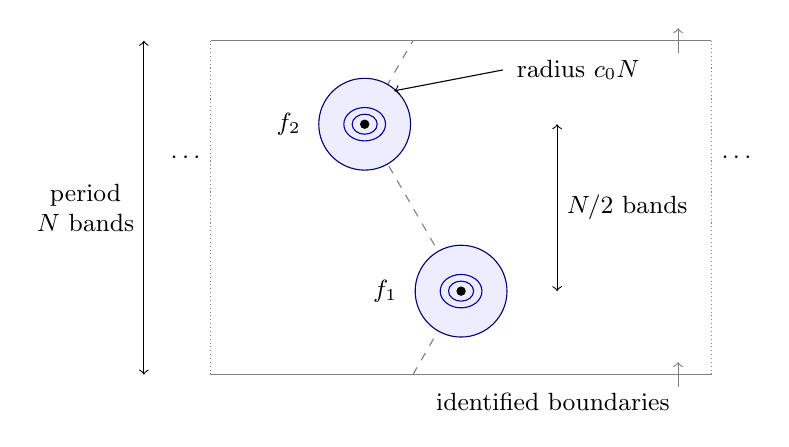
\begin{tikzpicture}[scale=1.06,every node/.style={font=\small}]
 \draw[gray] (-3,0)--(3,0) (-3,4)--(3,4);
 \draw[gray,densely dotted] (-3,0)--(-3,4) (3,0)--(3,4);
 \node at (-3.3,2.6) {$\cdots$};
 \node at (3.3,2.6) {$\cdots$};
 \draw[gray,dashed] (-.577,0)--(0,1)--(-1.155,3)--(-.577,4);
 \foreach \xx/\yy in {0/1,-1.155/3} {
   \fill[blue!7] (\xx,\yy) circle (.55);
   \draw[blue!45!black] (\xx,\yy) circle (.55);
   \draw[blue!65!black] (\xx,\yy) ellipse (.25 and .20);
   \draw[blue!65!black] (\xx,\yy) ellipse (.15 and .12);
   \fill (\xx,\yy) circle (1.6pt);
 }
 \node[left] at (-.65,1) {$f_1$};
 \node[left] at (-1.805,3) {$f_2$};
 \draw[<->] (1.15,1)--(1.15,3)
   node[midway,right] {$N/2$ bands};
 \draw[<->] (-3.8,0)--(-3.8,4)
   node[midway,left,align=center] {period\\$N$ bands};
 \draw[->,gray] (2.6,-.15)--(2.6,.15);
 \draw[->,gray] (2.6,3.85)--(2.6,4.15);
 \node[below] at (1.1,-.1) {identified boundaries};
 \draw[->] (.5,3.65)--(-.8,3.4);
 \node[right] at (.55,3.65) {radius $c_0N$};
\end{tikzpicture}
\caption{A schematic fundamental band of the cylinder, with the lattice
suppressed. The dashed column cut follows the two balanced row blocks;
its marked seams have displacement $-N/4+iN\sqrt3/4$ and are separated
vertically by half the period. For small fixed $c_0$,
their radius-$c_0N$ neighborhoods are disjoint and embed isometrically
in the plane. After essential and larger polygons are deleted at bounded
cost, each remaining polygon belongs to a nest in one of these two
neighborhoods. The independent choices give the square of the planar
partition in \eqref{eq:05-cylinder-planar-comparison}.}
\label{fig:E-planar-comparison}
\end{figure}

\begin{proof}
The two cylinder markers have disjoint neighborhoods of radius
\(c_0N\), each isometric to its planar neighborhood, if \(c_0\) is
small enough: along the standard balanced column cut their displacement
is \(-N/4+iN\sqrt3/4\), and their vertical separation is half the
balanced period.
Figure~\ref{fig:E-planar-comparison} shows the two embedded neighborhoods.
Delete all separating essential polygons, using
Proposition~\ref{prop:05-winding-suppression}, and all contractible
polygons of lifted diameter greater than \(c_0N\), using
Lemma~\ref{lem:05-macroscopic-removal} at both markers. The product of
the deletion costs is uniformly bounded.

Every remaining polygon is contractible and encloses exactly one marker
in its disk. A planar simple curve of diameter at most \(r\) enclosing a
point lies in the radius-\(r\) neighborhood of that point: the point is
in the curve's convex hull, so its distance to each curve point is at
most the curve's diameter. Hence each remaining polygon lies in its
marker's embedded neighborhood. Conversely, a planar nest counted by
\(P_\chi(c_0N)\) projects into that neighborhood and separates the
cylinder markers. The neighborhoods are disjoint, so the two nests can
be chosen independently. Retaining just these configurations gives the
lower bound, and the preceding deletion gives the upper bound in
\eqref{eq:05-cylinder-planar-comparison}.

For each fixed \(\chi>0\), Theorem~\ref{thm:04-cylinder-exponent} gives
\(Z_N(\chi)=N^{\tau(\chi)+o(1)}\) along even \(N\). Taking logarithms
in the comparison yields
\(P_\chi(c_0N)=N^{\tau(\chi)/2+o(1)}\). Monotonicity in the radius and
bracketing an arbitrary radius between consecutive admissible values
prove \eqref{eq:05-planar-all-fugacity}. At \(\chi=2\),
\(\tau(2)=1/6\), giving \eqref{eq:05-planar-nest-scaling}.
\end{proof}

\subsection{Nests around the middle of a strip}

Let \(S_k\) be the partition sum of nests around a face center \(f\)
on the middle line of the strip \(\mathcal S_{2k}\) of \(2k\) triangular
bands. Thus \(S_k\) sums the finite vertex-disjoint nests enclosing \(f\),
with weight \(\prod_P2\rho^{|P|}\), including the empty nest.

\begin{corollary}[Middle-face nesting]\label{E:strip-nesting}
As \(k\longrightarrow\infty\),
\begin{equation}
 S_k=k^{1/12+o(1)}.
 \label{eq:C-nest}
\end{equation}
\end{corollary}
\begin{proof}
Choose a fixed \(c_0>0\) so small that every nest enclosing \(f\),
with each polygon of diameter at most \(c_0k\), fits inside the strip. By
Lemma~\ref{lem:05-macroscopic-removal}, deleting all larger polygons
has a bounded cost. Therefore
\[
 P_2(c_0k)\le S_k\le C P_2(c_0k).
\]
Apply Theorem~\ref{thm:05-nest-normalization}.
\end{proof}

\subsection{A positive comparison between length and nests}

We use the boundary winding identity to count visits to one internal
edge by summing over all ordered boundary sources and endpoints. This
local comparison will convert the nesting exponent into a length
exponent. Recall \(t=3/8\), \(c=\cos(3\pi/8)\), and \(d=1/\sqrt2\).

For a finite simply connected union $D$ of triangular tiles with simple
polygonal boundary and a boundary port $a$, the boundary identity of \cite[Lemma~2.1]{StripCompanion} is
\begin{equation}\label{eq:E-boundary-input}
 \sum_{b\in\partial D}\sum_{\gamma:a\to b}
       \rho^{n(\gamma)}e^{itW(\gamma)}=1,
\end{equation}
where $W$ measures signed turning from the inward initial direction to
the outward final direction. Its local rule sends the current weight
into the two new continuations with multipliers
$\rho e^{i\lambda}$ and $\rho e^{-i\lambda}$; their sum is one.
At a first self-collision, reversing the closing cycle gives the
canceling winding increments $\pm4\pi/3$. In a convex domain every
boundary-to-boundary path satisfies $|W|\le\pi$, and therefore
$c\le\cos(tW)\le1$. These conventions also specify the modified
interior-source calculation below.


For a finite convex union $D$ of triangular tiles and an internal
honeycomb mid-edge $p$, define
\[
 L_p(D)=\sum_{a,b\in\partial D}\ \sum_{\gamma:a\to b}
 \rho^{n(\gamma)}\cos(tW(\gamma))\,
 \mathbf1_{\{p\in\gamma\}}.
\]
The boundary ports are ordered, and $W(\gamma)$ is the total signed
turning from the initial inward direction to the final outward direction.
Convexity gives $c\le\cos(tW(\gamma))\le1$.
For a point $r$ not on a polygon, let $\mathcal Z_r(D)$ be the sum over
finite sets of pairwise vertex-disjoint simple polygons, all strictly
enclosing $r$, with weight $\prod_\ell 2\rho^{|\ell|}$; the empty set
has weight one. The same definition applies when $r$ is a mid-edge,
excluding polygons through that mid-edge.

\begin{lemma}[Length and polygon nests]\label{lem:02-length-nests}\label{E:length-nest}
Let $f_1,f_2$ be the two honeycomb face centers adjacent to $p$. Then
\[
 d\bigl(\mathcal Z_{f_1}(D)+\mathcal Z_{f_2}(D)\bigr)
 \le L_p(D)\le
 \mathcal Z_{f_1}(D)+\mathcal Z_{f_2}(D).
\]
The inequalities also hold, with finite quantities, in every homogeneous
infinite strip of fixed positive height.
\end{lemma}
\begin{proof}
Cut the edge at $p$ into two stopping outlets. For a boundary source
$a$, the winding splitting identity still has total one: every collision
stem approaches its closing cycle from outside, so the two orientations
cancel. Subtract this identity from the one without the cut. The total
winding weight of paths visiting $p$ equals that of paths from $a$
stopping at the cut. Reversing these paths and taking real parts gives
$L_p(D)=F_+(D)+F_-(D)$, where $F_\sigma$ is the real winding-weighted
sum of paths from the specified side $p^\sigma$ to the exterior. The
initial direction points into the neighboring vertex on that side.

Apply the same splitting procedure from this interior source, retaining
all stopping possibilities. A return to the other side of the cut traces
a polygon $\ell'$ through $p$. For a fixed initial side it is counted
once and has turning $\pm2\pi$, hence real factor
$\cos(2\pi t)=-d$. A collision with a polygon not enclosing $p$
cancels with its reversed orientation. If its polygon $\ell$ strictly
encloses $p$, the stem approaches from inside. The closing turn of the
counterclockwise polygon at the collision vertex is $-\pi/3$, whereas
the turn from the stem into that orientation is $+\pi/3$. The added
winding is therefore $8\pi/3$, or $-8\pi/3$ for the other orientation.
Both have factor $\exp(\pm it8\pi/3)=-1$.

For a fixed enclosing $\ell$, sum the stems in its interior, excluding
its vertices. This is exactly the corresponding $F_\sigma$ for the
smaller domain: the stem stops at the mid-edge before its aimed-at
vertex, whose weight belongs to $\ell$. If its initial direction already
points at an excluded vertex, this stem sum is one. No further inner
polygon is then possible. Write \(D_\ell\) for the domain strictly inside an enclosing polygon
\(\ell\), with its vertices excluded and with stopping outlets on the
incident half-edges. Conservation of the initial mass, followed by the
collision classification above, gives the recurrence
\[
 F_\sigma(D)=1+d\sum_{\ell'\ni p}\rho^{|\ell'|}
       +2\sum_{\ell\text{ enclosing }p}\rho^{|\ell|}F_\sigma(D_\ell).
\]
The factor two in the last sum comes from the two orientations of the
enclosing polygon, each with real factor \(-1\) on the stopped side
of the conservation identity. The initial-source convention just
specified gives \(F_\sigma(D_\ell)=1\) if its first vertex is excluded.

Iterate this recurrence, choosing an outermost enclosing polygon first
and then polygons strictly inside it. Every nested family is obtained
once in this order. The iteration terminates either with the constant
term one or with a polygon through \(p\); such a polygon must be the
innermost selected cycle: \(p\) lies on its boundary, so no disjoint
cycle strictly inside its bounded disk can enclose \(p\). Every enclosing cycle removes vertices,
so the iteration is finite. It gives, for either sign,
\[
 F_\sigma(D)=\mathcal Z_p(D)+d\sum_{\ell'\ni p}
       \rho^{|\ell'|}\mathcal Z_{\mathrm{around}}(\ell'),
\]
where $\mathcal Z_{\mathrm{around}}(\ell')$ sums the disjoint outer
polygons surrounding $\ell'$, with fugacity two per polygon. This
recursion remains valid if the opposite neighbor of $p$ is excluded;
in that case there is no return to the cut.

A polygon enclosing exactly one of $f_1,f_2$ uses their separating
edge. There can be at most one such polygon in a disjoint nest, and it
is the innermost polygon of that nest: any smaller polygon around the
same face would also have to use that edge. Consequently
\[
 \mathcal Z_{f_1}(D)+\mathcal Z_{f_2}(D)
 =2\mathcal Z_p(D)+2\sum_{\ell'\ni p}
       \rho^{|\ell'|}\mathcal Z_{\mathrm{around}}(\ell').
\]
Together with the preceding expression for $F_++F_-$ and $0<d<1$,
this proves the finite-domain claim.

Exhaust an infinite strip by parallelograms. The top/bottom path sums
and the nesting sums increase. The terms with a distant side-wall
endpoint tend to zero. To justify the latter assertion, split a path
at $p$ and discard avoidance between its arms. Keep a fixed group of
columns containing $p$. On either side, the vacuum transfer supplies
a uniformly bounded half-state. A top/bottom endpoint is bounded by
the sum over its source column followed by one-defect propagation to
the fixed columns; this sum converges by the fixed-height transfer
decay. A side-wall endpoint contributes a decaying one-defect power,
with only finitely many wall ports. Thus each arm is uniformly summable
and its side-wall part tends to zero. The upper bound on $L_p$ obtained
in this way and the lower finite-domain inequality also prove finiteness
of the limiting nesting sums.
\end{proof}


\subsection{Raw and conditioned first-length estimates}

We now keep a single bottom boundary port \(a\) fixed. Let
\(\mathcal P_N(a)\) be the self-avoiding port paths in the open
\(N\)-band strip from \(a\) to either boundary, with no other boundary
visit. These are the bottom arches and the bridges. Their terminal
ports are summed over their actual lattice positions; there is no
additional translation sum. Write
\[
 \mathcal M_N(a)=\sum_{\gamma\in\mathcal P_N(a)}
                  \rho^{n(\gamma)}n(\gamma),
\]
where \(n(\gamma)\) counts visited honeycomb vertices. This is an
unnormalized first-length mass.

\begin{proposition}[Raw first-length mass]\label{E:raw-first-moment}
There is a constant \(C\), independent of the boundary source and
\(N\ge1\), such that
\begin{equation}
 \mathcal M_N(a)\le C(1+NS_{N+1})
                      \le N^{13/12+o(1)}
 \qquad(N\longrightarrow\infty).
 \label{eq:05-raw-first-moment}
\end{equation}
\end{proposition}
\begin{proof}
Sum \(L_p(\mathcal S_N)\) over one representative of each internal
mid-edge orbit under integer horizontal translation. For each summand, translate its source port to the fixed representative
of its boundary orbit. The marked internal edge then runs through all
visits of the translated path. This is a bijection between the two sets
of path--edge pairs, preserving both length and winding; hence translation
invariance turns the sum into the winding-weighted number of internal
edge visits for paths from the chosen source representatives.
There is one bottom-port orbit and one top-port orbit, whose source
totals agree by a half-turn. Thus, if \(\mathcal E_N\) is the chosen
set of internal mid-edge representatives, the orbit-count identity is
\[
 \sum_{p\in\mathcal E_N}L_p(\mathcal S_N)
 =2\sum_{\gamma\in\mathcal P_N(a)}
       \rho^{n(\gamma)}(n(\gamma)-1)\cos(tW(\gamma)).
\]
A path with \(n\) vertices has \(n-1\) internal mid-edge visits, and
its winding cosine is between \(c\) and one. There are \(O(N)\)
internal edge orbits. These positive sums may be rearranged by monotone
convergence.

Every face-center nesting mass in the strip is at most \(S_{N+1}\):
embed the strip in a \(2(N+1)\)-band strip whose middle line contains
the chosen face center. Lemma~\ref{lem:02-length-nests} now bounds the
sum of internal edge visits by \(CNS_{N+1}\). To replace \(n-1\) by
\(n\), add the boundary partition mass
\(\mathcal A_N+\mathcal B_N\le 1/c\), using the strip identity
\(c\mathcal A_N+\mathcal B_N=1\). This proves the first inequality;
Corollary~\ref{E:strip-nesting} proves its asymptotic form.
\end{proof}

\begin{proposition}[Length conditional on reaching macroscopic height]
\label{prop:02-length-reduction}
Give \(\mathcal P_N(a)\) its normalized critical weights. Conditional
on the path reaching the top boundary of the bottom
\(\lfloor N/4\rfloor\) bands, its
expected number of visited vertices is \(N^{4/3+o(1)}\).
\end{proposition}
\begin{proof}
Put \(k=\lfloor N/4\rfloor\), and take \(N\) large enough that
\(k\ge1\). A path is confined to the bottom \(k\)-band strip exactly
when it stays below its top line: crossing that line uses a port between
the two adjacent bands. Thus the conditioning event consists of all
bridges and precisely the bottom arches not counted by \(\mathcal A_k\).
Its unnormalized mass is
\[
 q_N=\mathcal B_N+\mathcal A_N-\mathcal A_k
     =\mathcal B_k/c-(1/c-1)\mathcal B_N
     \asymp N^{-1/4}.
\]
Indeed monotonicity gives
\(\mathcal B_k\le q_N\le\mathcal B_k/c\), and the strip theorem gives
\(\mathcal B_k\asymp N^{-1/4}\).

Restrict the orbit sum in the preceding proof to internal mid-edges
whose heights lie in the central third. For sufficiently large \(N\),
each adjacent face center is at distance at least \(N/3-O(1)>k\)
bands from either boundary. Its centered \(2k\)-band strip therefore
fits inside \(\mathcal S_N\), so its nesting mass is at least \(S_k\).
There are at least \(c_1N\) such internal edge orbits, and
Lemma~\ref{lem:02-length-nests} gives a lower bound \(c_2NS_k\) for
their total winding-weighted visit mass. Any bottom-source path counted
there reaches the top boundary of the bottom \(k\) bands; the rotated statement holds
for a top source. Since the winding cosine is at most one and the
number of counted visits is at most the path length, the unnormalized
first-length mass of the conditioning event is at least \(c_3NS_k\).
Its upper bound is \(\mathcal M_N(a)\). By
Corollary~\ref{E:strip-nesting} and
Proposition~\ref{E:raw-first-moment}, these bounds both have exponent
\(13/12\). Division by \(q_N\) gives
\(N^{13/12+1/4+o(1)}=N^{4/3+o(1)}\).
\end{proof}
